\section{Descrizione e motivazioni delle tecnologie adottate }
In questa sezione vengono presentate le tecnologie adottate per l’implementazione delle componenti client e server del sistema.
Inoltre, vengono descritte le architetture specifiche utilizzate nel back-end, in relazione alle tecnologie impiegate, e quelle adottate nel front-end.

\subsection{Tecnologie e architettura backend}
L'architettura del nostro server è stata progettata per rispondere alle esigenze richieste dal cliente, dove è stata prioritizzata la velocità di sviluppo e deployment senza sacrificare robustezza e sicurezza. Abbiamo adottato un'architettura \textbf{monolitica} basata su una struttura a livelli, che facilita la separazione delle responsabilità e garantisce una maggiore manutenibilità nel tempo. La scelta di un'architettura monolitica si giustifica con la necessità di ridurre la complessità iniziale e non rallentare lo sviluppo, mantenendo comunque una struttura modulare che potrà essere facilmente evoluta nel tempo, ad esempio, trasformando parti del sistema in microservizi qualora il progetto dovesse espandersi in futuro.
\\
Le tecnologie selezionate per lo sviluppo del backend sono state scelte in base a una combinazione di familiarità e facilità d'uso, con l'obiettivo di accelerare il processo di implementazione e garantire al contempo solidità e qualità del codice.
\\
Il back-end è stato sviluppato utilizzando \textbf{Spring Boot}, abbiamo optato per questo framework grazie alle sue numerose configurazioni predefinite e utili estensioni come \textbf{Lombok}, che ci permettono di concentrarci sulla logica di business anziché su complesse configurazioni di sistema o codice ripetuto. Spring Boot consente di avviare rapidamente un'applicazione web robusta e scalabile.
esso sono state integrate diverse tecnologie complementari, tra cui:

\begin{itemize}
	\item \textbf{Hibernate}: Per la gestione della persistenza, Hibernate si rivela una scelta efficace, in quanto astrae le operazioni di accesso al database e riduce significativamente il lavoro manuale nella scrittura di query SQL. Questo approccio rende il codice più leggibile e facilmente mantenibile.
	
	\item \textbf{Spring Security e JWT (JSON Web Token)}: Per garantire un'autenticazione stateless e sicura, abbiamo deciso di utilizzare i JWT. Questa soluzione permette di gestire le sessioni degli utenti in maniera efficiente, differenziando eventuali ruoli o permessi e riducendo il carico sul server.
	
	\item \textbf{Jackson}: È uno strumento potente per serializzare e deserializzare oggetti Java in \textbf{JSON} e viceversa.
	Quando si utilizza l’annotazione \colorbox{lightgray}{@RestController} o \colorbox{lightgray}{@ResponseBody}, Spring Boot restituisce automaticamente le risposte in formato JSON senza necessità di configurazioni aggiuntive.
	
	\item \textbf{Swagger}: L’adozione di Swagger per la documentazione delle REST API agevola notevolmente il testing e la verifica degli endpoint, creando al contempo una documentazione ricca di informazioni utili per condividere informazioni critiche.
\end{itemize}

Il back-end del sistema segue il pattern architetturale \textbf{MVC (Model-View-Controller)}, nativamente supportato dal framework \textbf{Spring Boot}.
Nel nostro caso, il \textbf{Model} è rappresentato dalle entità e dalla logica di business implementata nei servizi; il \textbf{Controller} è costituito dai componenti RESTful che gestiscono e mappano le richieste HTTP.
La \textbf{View} non è gestita all’interno del back-end, poiché l’applicazione svolge il ruolo di \textbf{API REST}, restituendo risposte in formato JSON al client, che si occupa della rappresentazione dei dati.
Questo approccio garantisce una chiara \textbf{separazione delle responsabilità}, migliorando la \textbf{modularità} e la \textbf{manutenibilità} del sistema.
\\ \\
Di seguito viene riportato uno schema del design utilizzato del backend

\begin{figure}[H]
	\centering
	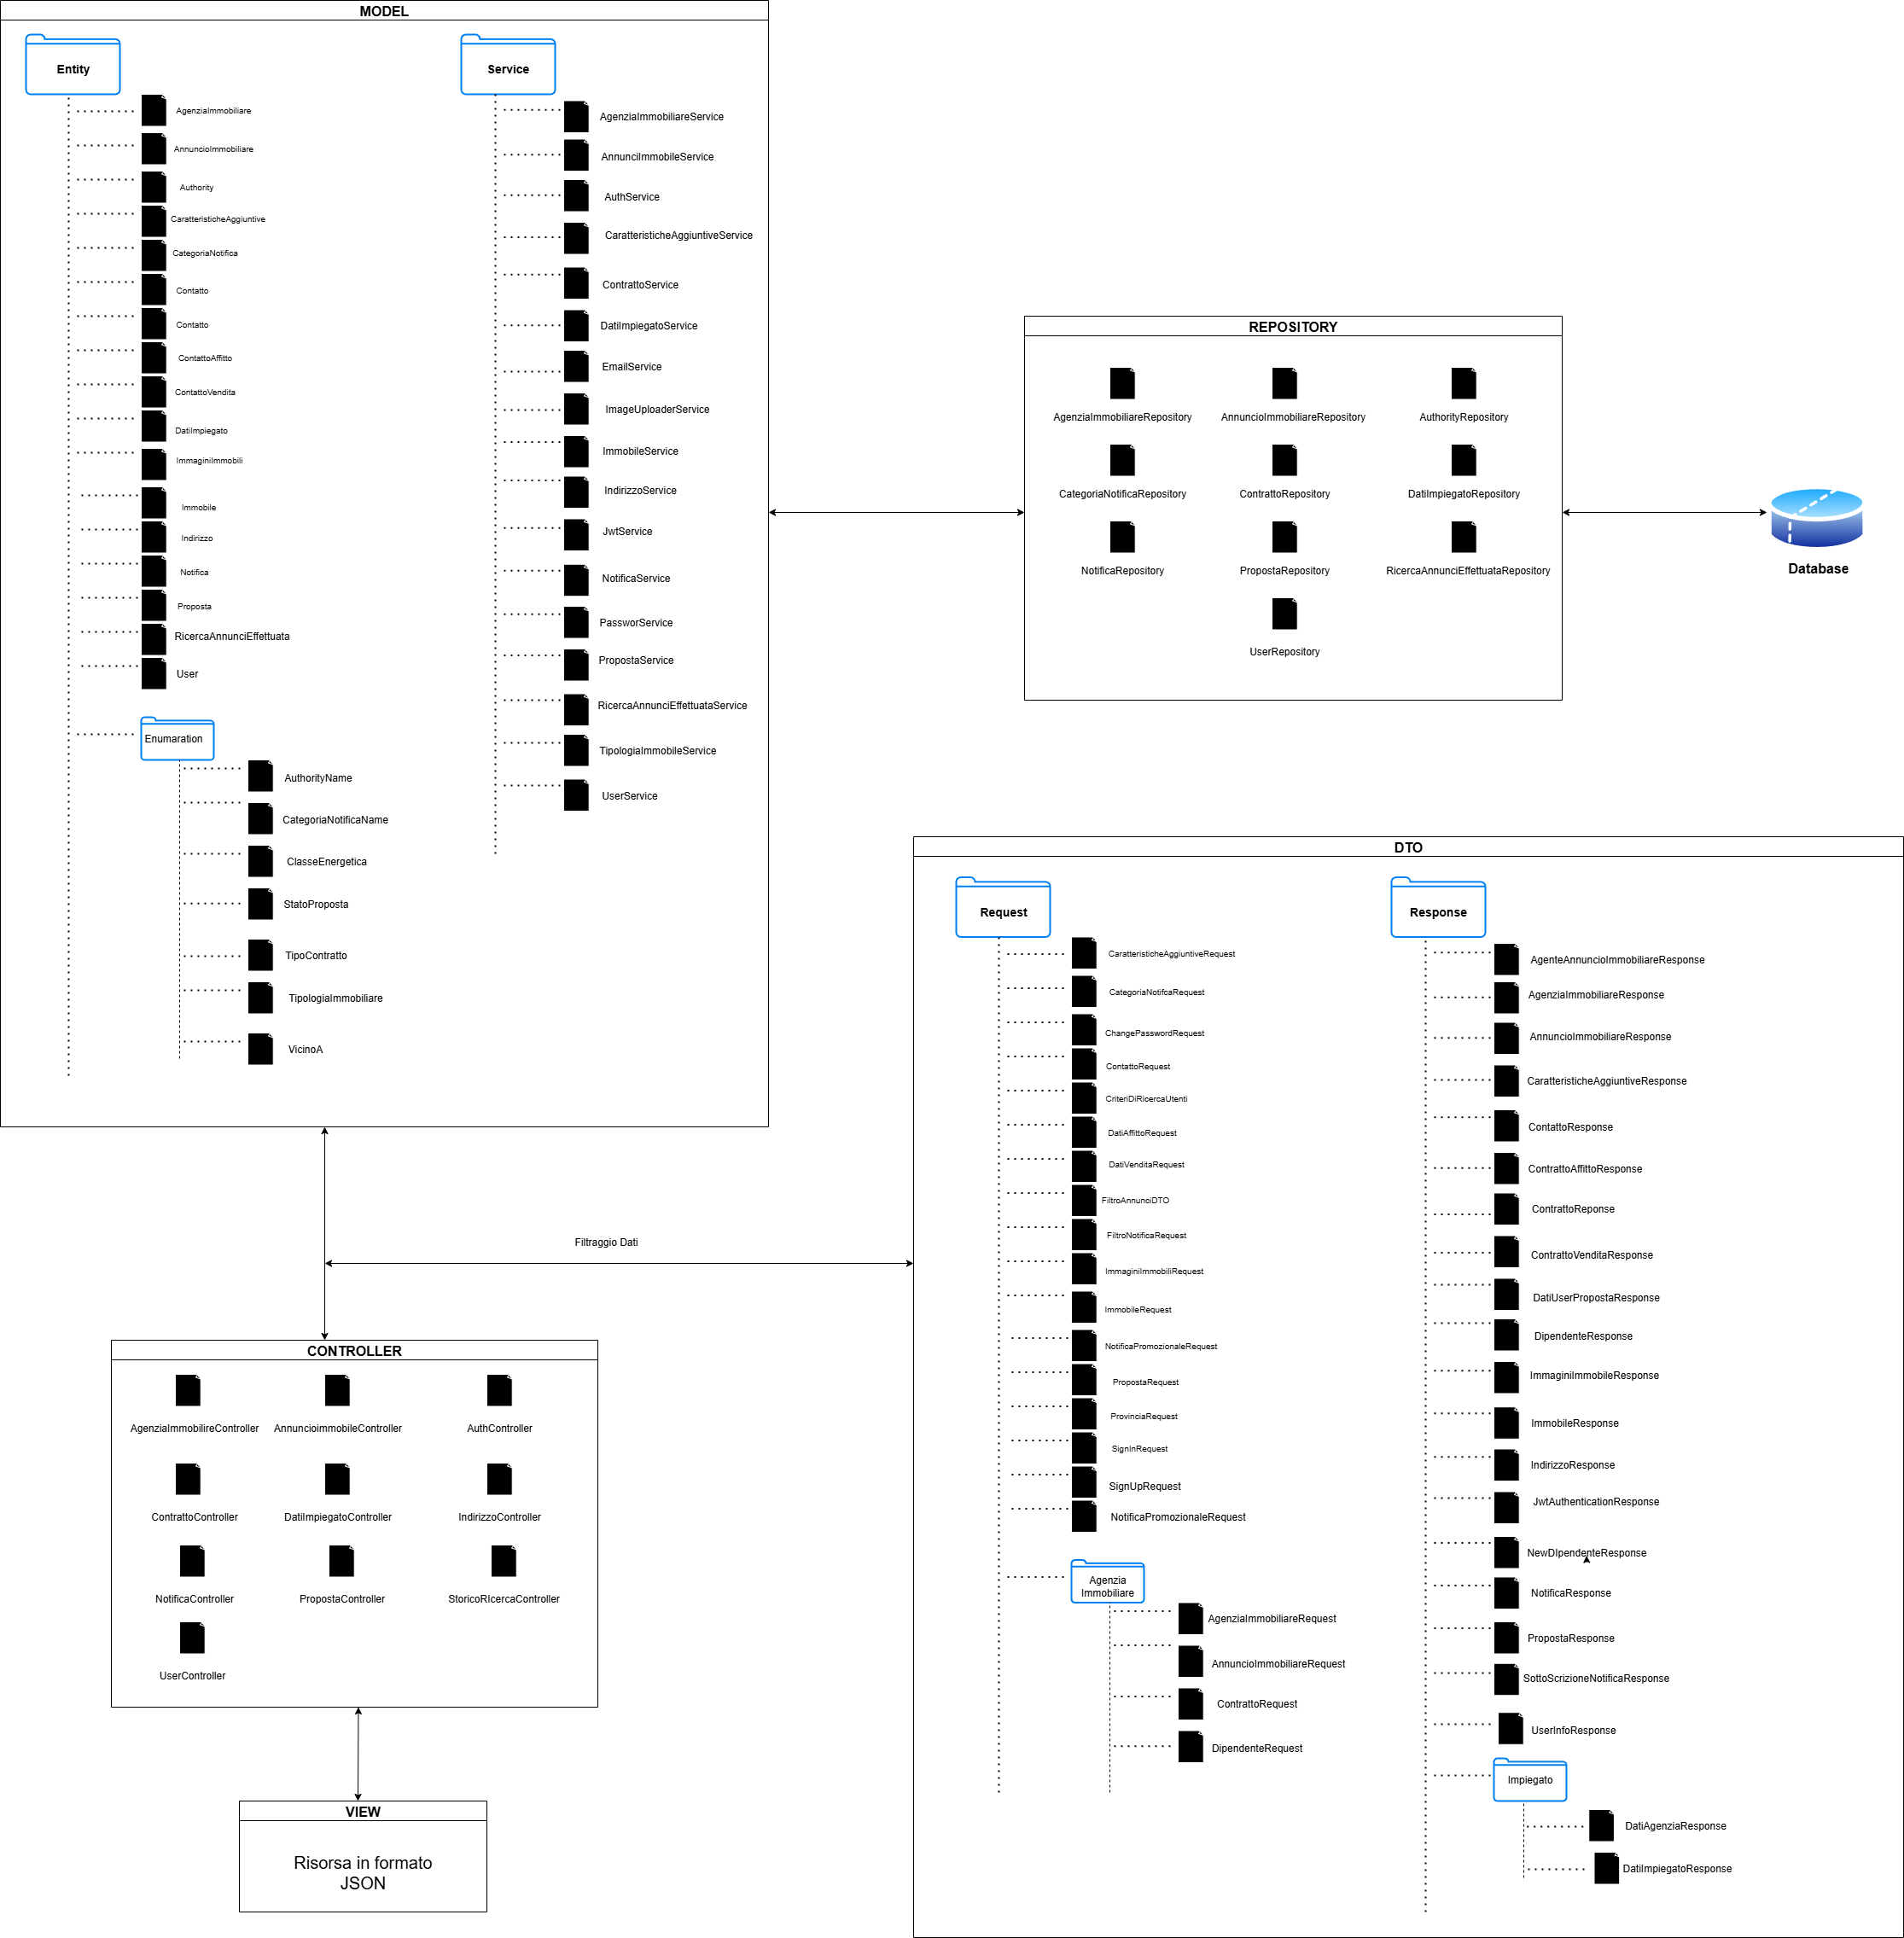
\includegraphics[width=1\linewidth]{Immagini/Schema backend.png}
	\caption[schema backend]{Schema sintetico dell'architettura del backend}
\end{figure}

\begin{itemize}
	
	\item \textbf{MODEL}: Il Modello rappresenta i dati e la logica di business dell’applicazione, indipendentemente da come questi dati vengano visualizzati. In un’architettura MVC, il modello non deve dipendere dalle viste né dai controller, ma deve fornire metodi che consentano ai \textbf{controller} di manipolare i dati in risposta alle richieste dell’utente. Nel contesto del
	nostro sistema, il package \textbf{Service} all’interno del Model offre i metodi necessari per la 22 manipolazione dei dati relativi alle entità. Queste entità, grazie alle \textbf{funzionalità di Spring Boot}, sono mappate automaticamente alle relative tabelle nel database, facilitando l’interazione con i dati persistenti. L’accesso ai dati avviene tramite il \textbf{repository}, che permette di recuperare le informazioni direttamente dal database.
	
	\item \textbf{CONTROLLER}:  Il Controller svolge un ruolo fondamentale nell’architettura MVC come \textbf{ponte tra il Model e la View}. In particolare, gestisce le interazioni dell’utente, elabora le richieste e aggiorna sia il Model che la View in base alle azioni dell’utente.
	Quando un utente interagisce con l’interfaccia (la View), il Controller riceve l’input, elabora i dati (eventualmente tramite il Model, che contiene la logica di business) e quindi
	aggiorna la View per riflettere i cambiamenti dello stato. Nel nostro sistema, che segue l’architettura \textbf{RESTful API}, l’input dell’utente è rappresentato dalle richieste \textbf{HTTP (come POST, GET, PUT, DELETE)}. Ogni Controller gestisce le richieste relative a una specifica entità (ad esempio, UserController, AgenziaImmobiliareController, ecc.) e quindi si occupa di ricevere e rispondere a queste richieste. Una particolarità del nostro sistema è l’uso di \textbf{DTO (Data Transfer Object)}, che funge da \textbf{strato di filtraggio} tra la logica di business (Model) e le risposte al client. Le DTO vengono utilizzate per limitare i dati che vengono passati nelle richieste e nelle risposte. In altre parole, quando un client invia una richiesta al Controller o quando il Controller restituisce una risposta, la DTO permette di selezionare solo le informazioni necessarie, evitando di esporre direttamente l’intera entità. Questo approccio migliora la \textbf{sicurezza} e l’\textbf{efficienza}, poiché impedisce di passare dati non necessari e riduce il rischio di esposizione di informazioni sensibili. Per esempio, se un’entità Utente ha campi come id, nome, email, password, il Controller potrebbe rispondere con una DTO che include solo i campi nome ed email, evitando di restituire campi sensibili come la password. In questo modo, solo le informazioni realmente necessarie per il client vengono trasmesse.
	
	\item \textbf{VIEW}: La View è responsabile della \textbf{rappresentazione grafica dei dati} e dell’interfaccia utente. Poiché il nostro back-end è un’architettura \textbf{API RESTful}, la View viene gestita interamente dal client.
	
\end{itemize}

Il sistema include ulteriori pacchetti che contengono classi di configurazioni o classi di ausilio: 

\begin{itemize}
	
	\item In \textbf{config} troviamo le classi necessari per la configurazione del framework e la gestione della sicurezza, come l’autenticazione, essenziale per garantire l’accesso controllato agli end-point e il corretto esito delle risposte
	HTTP. Ad esempio, gli end-point che iniziano con \colorbox{lightgray}{/pb} sono configurati come accessibili liberamente, senza necessità di autenticazione. Questa impostazione viene definita nel file \textbf{SecurityConfiguration}, situato all’interno.
	
	\item In \textbf{exception} ci sono le classi che estendono RunTimeException.
	Ogni eccezione personalizzata rappresenta uno specifico stato di errore HTTP restituito nella risposta. La classe \colorbox{lightgray}{ExceptionManagement} gestisce tutte le eccezioni personalizzate, mappandole sul corretto codice di errore HTTP al momento del loro lancio.
	
	\item In \textbf{utils} contiene classi che offrono metodi statici di utilità riutilizzabili dai componenti del livello service. 
	In particolare \colorbox{lightgray}{getUserCurrent()} della classe UserContex, ampiamente utilizzato per ottenere l’utente che ha effettuato una richiesta HTTP tramite il contesto di sicurezza di Spring (SecurityContext).
	
	\item Infine rimangono i package \textbf{factory} e \textbf{strategy} contengono le classi di supporto ai service responsabili dell’invio di notifiche agli utenti, generando dinamicamente il contenuto in base alla categoria della notifica. Tale esigenza è stata risolta applicando il \textbf{pattern Factory Method}, che prevede la definizione di una \textbf{interfaccia comune} e di \textbf{classi factory specifiche} in grado di restituire l’istanza più appropriata in base al contesto.
	In combinazione, il \textbf{pattern Strategy} consente di definire comportamenti diversi per la generazione del contenuto della notifica, migliorando flessibilità e manutenibilità del sistema.
	
\end{itemize}
 
\subsection{Tecnologie e architettura frontend}

Poiché il sistema adotta un’architettura client-server, lo sviluppo del client è completamente indipendente dal server.
In questa prospettiva, abbiamo scelto di realizzare un’applicazione web-based, utilizzando tecnologie front-end moderne per garantire un’esperienza utente fluida e reattiva.
Tale approccio consente di mantenere una netta separazione tra logica di presentazione e logica applicativa, e permette, in futuro, di sviluppare ulteriori client, come un’applicazione mobile, che potranno interagire con lo stesso server senza necessità di modificarne l’implementazione.
\\ \\
È stato adottato il \textbf{framework Vue.js}, una libreria basata su JavaScript progettata per la costruzione di interfacce utente dinamiche e reattive. Vue.js è particolarmente
indicato per lo sviluppo di applicazioni \textbf{Single-Page Application (SPA)}, ossia applicazioni web che offrono un’esperienza utente fluida, simile a quella delle applicazioni desktop. \\
Le SPA permettono agli utenti di interagire con un sito o un’applicazione senza dover ricaricare l’intera pagina, grazie alla gestione dinamica dei contenuti attraverso JavaScript. Questo
approccio riduce i tempi di caricamento e migliora la responsività dell’interfaccia, risultando
particolarmente utile per sistemi complessi come quello sviluppato nel nostro progetto.
\\ \\

Di seguito viene presentato uno schema del fronend, seguito da una discussione approfondita delle strategie progettuali e delle tecnologie utilizzate.

\begin{figure}[H]
	\centering
	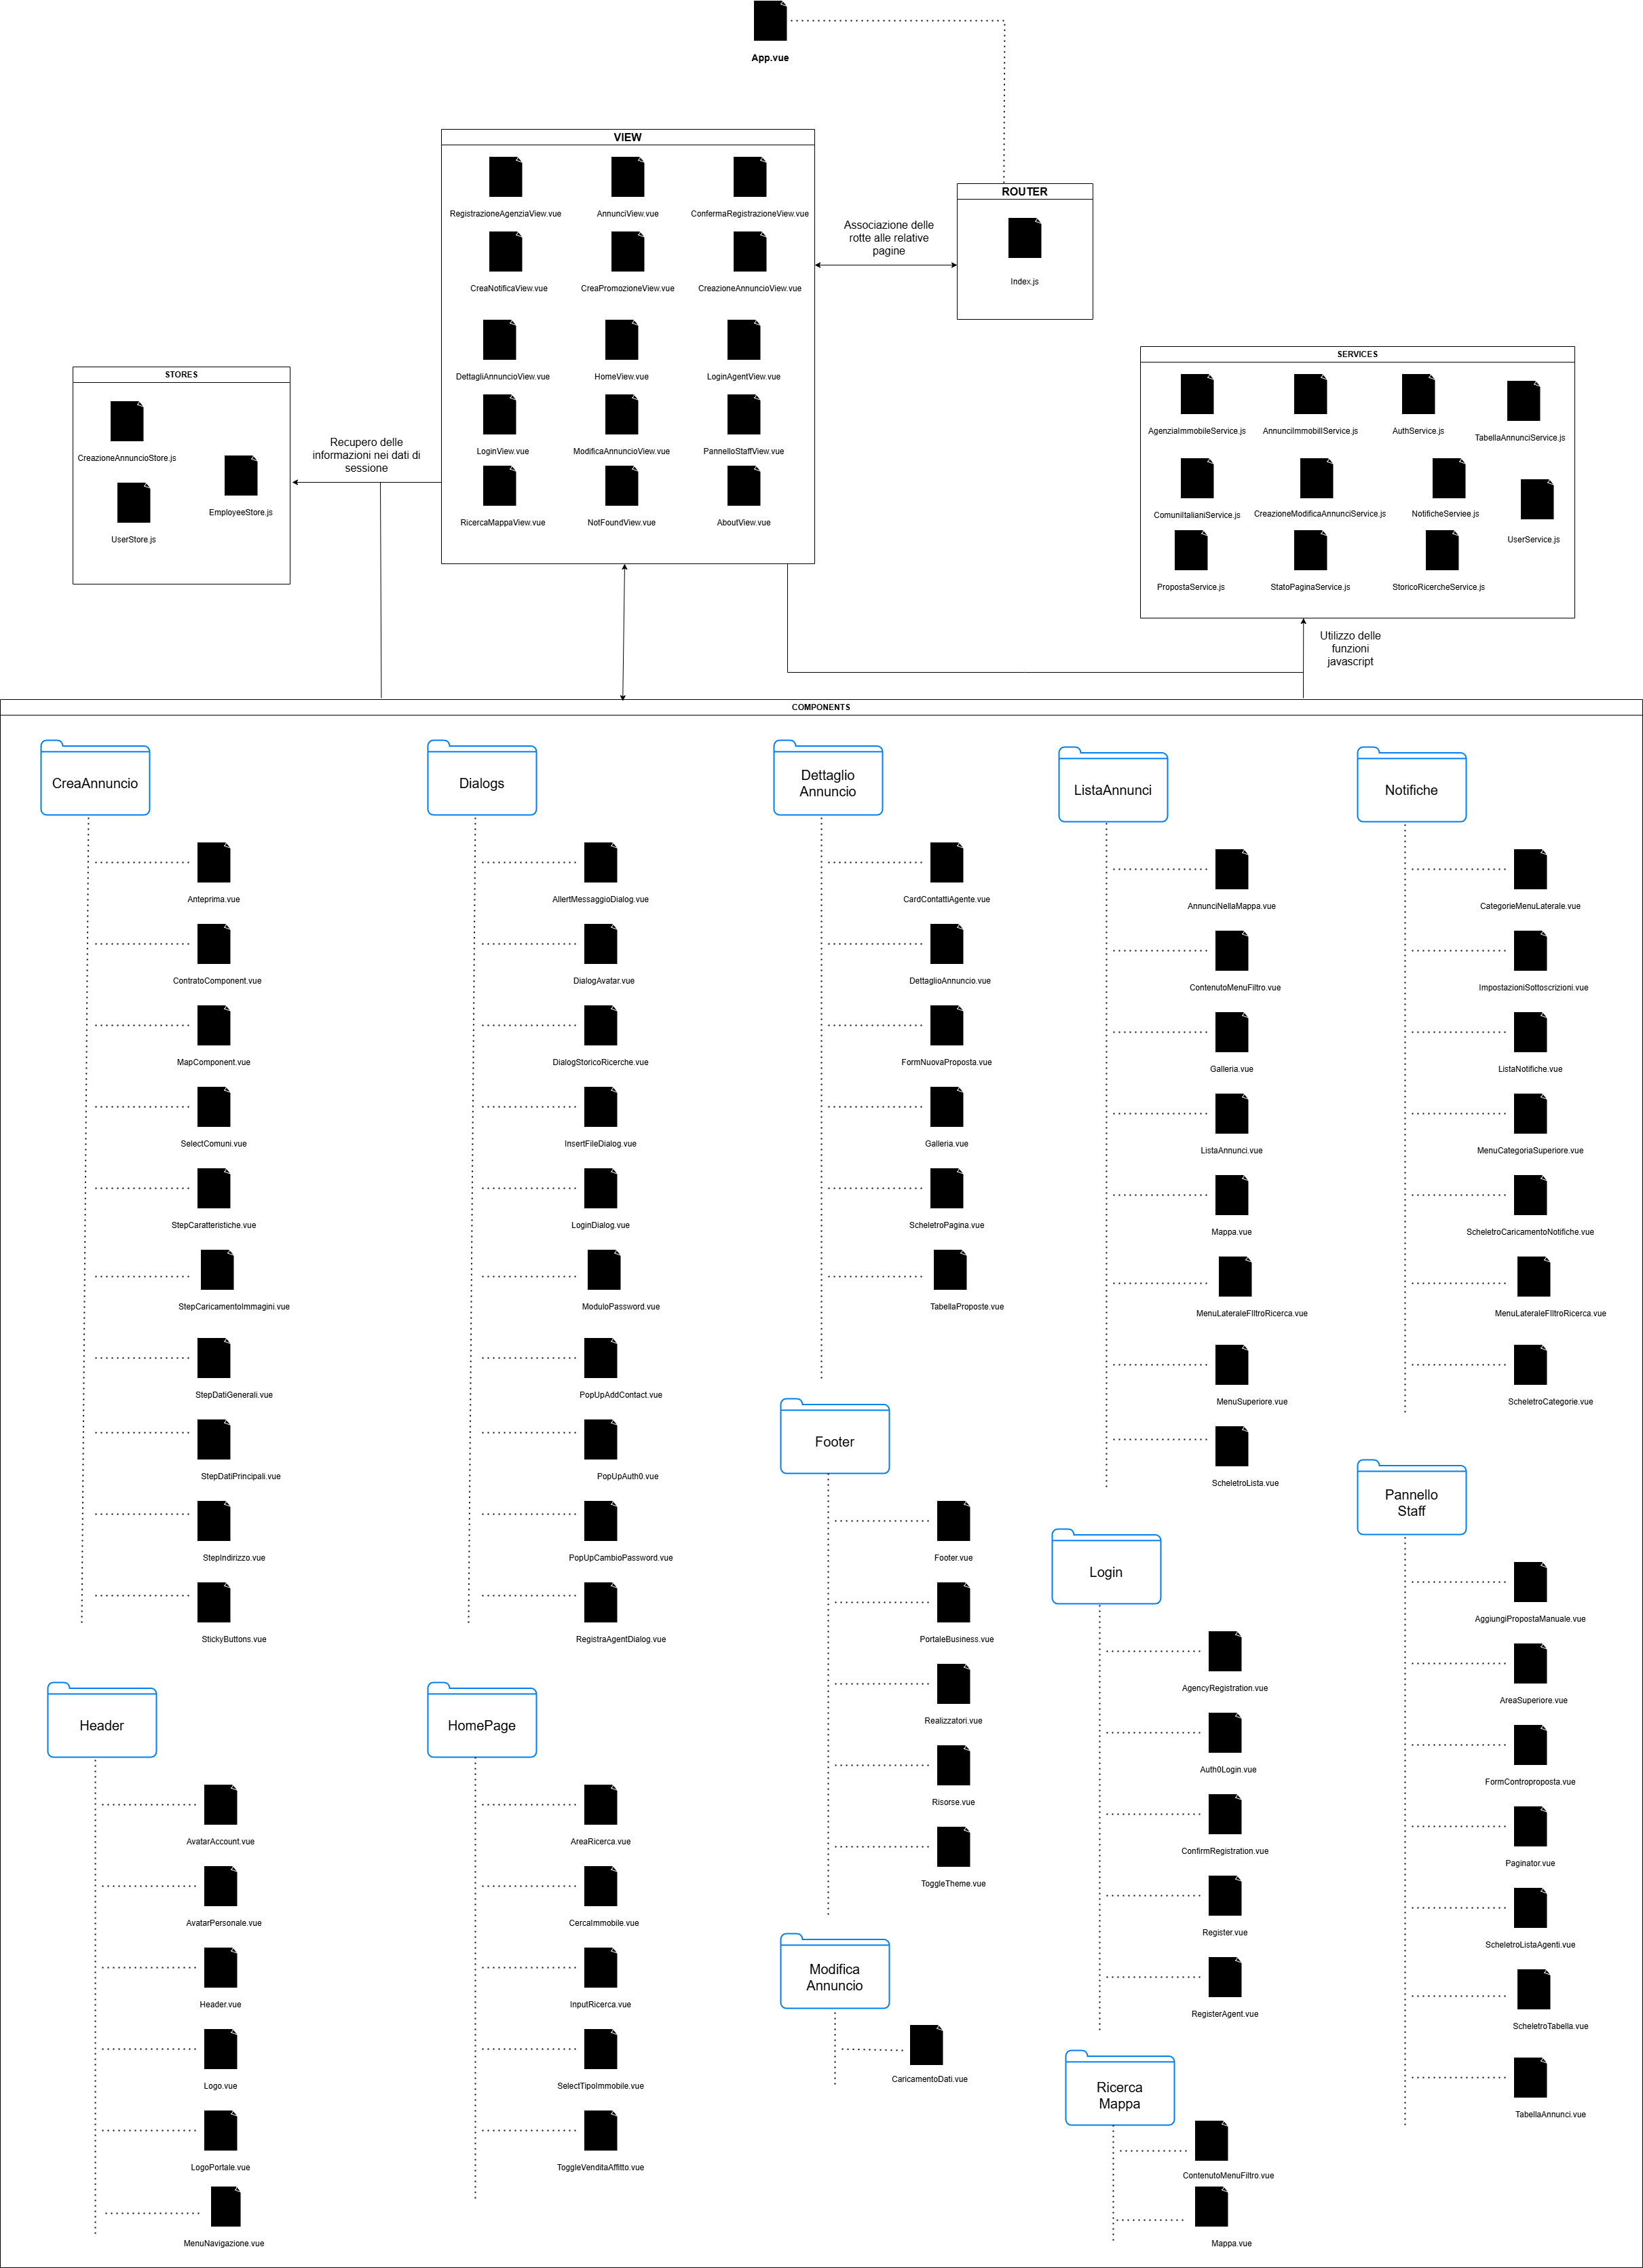
\includegraphics[width=1\linewidth]{Immagini/Schema frontend.png}
	\caption[Schema frontend]{Schema sintetico dell'architettura del frontend}
\end{figure}

Il codice sorgente del client è organizzato nel package src, che contiene i file principali dell’applicazione
e la configurazione del framework Vue.js. Le dipendenze del progetto, installate tramite npm, si trovano nella directory node\_modules. Di seguito illustriamo le componenti presenti in src:

\begin{itemize}
	
	\item \textbf{App.vue}: L’inizializzazione del framework parte dal file \colorbox{lightgray}{App.vue}, che funge da punto di ingresso per l’applicazione. All’interno di questo file vengono configurate le \textbf{componenti principali} e definito il sistema di routing, che sarà descritto in dettaglio nel punto successivo.
	In particolare, sono presenti le componenti \colorbox{lightgray}{Header} e \colorbox{lightgray}{Footer}, posizionate rispettivamente nella parte superiore e inferiore dell’interfaccia.
	Queste componenti sono incluse nel file principale poiché risultano \textbf{sempre visibili}, indipendentemente dalla pagina in cui si trova l’utente. Inoltre, la direttiva \colorbox{lightgray}{<router-view>} consente di visualizzare dinamicamente la vista corretta in base all’URL richiesto.
	In questa fase viene anche verificato se l’utente autenticato appartiene al ruolo di \textbf{membro} o di {staff}: in quest’ultimo caso, l’applicazione reindirizza automaticamente l’utente alla sezione riservata al personale.
	
	\item \textbf{Directory View}: La directory views contiene tutti i file \textbf{vue} che rappresentano le pagine principali del sito e sono associati a specifiche rotte tramite il sistema di routing.
	Come accennato in precedenza, Vue.js permette la creazione di \textbf{Single-Page Application (SPA)}, ma queste applicazioni presentano lo svantaggio di non avere una suddivisione naturale in pagine, compromettendo la navigabilità. Per risolvere questo problema, utilizziamo la libreria ufficiale \textbf{Vue Router}, che consente di associare un URL (o rotta) a una specifica view.
	
	\item \textbf{Directory router}: La directory router contiene un unico file index.js, in cui viene configurato il sistema di routing dell’applicazione. In questa configurazione, ogni rotta è associata alla rispettiva view descritta sopra, garantendo la navigazione fluida e dinamica tipica delle SPA.
	
	\item \textbf{Directory components}: La directory components contiene tutti i file .vue che rappresentano le componenti riutilizzabili dell’applicazione. A differenza della directory views,
	dove le view corrispondono alle pagine principali e sono direttamente associate alle rotte
	tramite il router, qui troviamo una suddivisione logica di elementi più granulari che vengono richiamati all’interno delle view. Le componenti in questa directory servono a fornire
	modularità al codice, favorendo la riutilizzabilità e una manutenzione più semplice. Inoltre
	implementano funzionalità specifiche che possono essere combinate per costruire view più
	complesse. Le componenti in questa directory non sono associate direttamente alle rotte
	ma vengono importate e utilizzate nelle rispettive view, garantendo un’organizzazione
	logica e semplificando la struttura complessiva del progetto.
	
	\item \textbf{Directory Service}: La directory service contiene file JavaScript che implementano funzioni e logiche riutilizzabili, progettate per essere utilizzate nelle diverse componenti dell’applicazione. Le operazioni ripetitive o complesse, come il recupero di dati da un server o la formattazione di informazioni, sono centralizzate in questa directory.
	
	\item \textbf{Directory stores}: La directory stores contiene file JavaScript che utilizzano \textbf{Pinia}, una libreria ufficiale di Vue.js per la gestione dello stato. Questa struttura permette di salvare informazioni a livello di sessione e di renderle facilmente accessibili in diverse parti dell’applicazione. Grazie a Pinia, le informazioni archiviate possono essere recuperate localmente, riducendo il tempo necessario per caricare dati critici.
	
\end{itemize}